\documentclass[12pt]{article}
\usepackage[margin=2.5cm]{geometry}
\usepackage{enumerate}
\usepackage{amsfonts}
\usepackage{amsmath}
\usepackage{fancyhdr}
\usepackage{amsmath}
\usepackage{amssymb}
\usepackage{amsthm}
\usepackage{mdframed}
\usepackage{graphicx}
\usepackage{subcaption}
\usepackage{adjustbox}
\usepackage{listings}
\usepackage{xcolor}
\usepackage{booktabs}
\usepackage[utf]{kotex}

\definecolor{codegreen}{rgb}{0,0.6,0}
\definecolor{codegray}{rgb}{0.5,0.5,0.5}
\definecolor{codepurple}{rgb}{0.58,0,0.82}
\definecolor{backcolour}{rgb}{0.95,0.95,0.92}

\lstdefinestyle{mystyle}{
    backgroundcolor=\color{backcolour},
    commentstyle=\color{codegreen},
    keywordstyle=\color{magenta},
    numberstyle=\tiny\color{codegray},
    stringstyle=\color{codepurple},
    basicstyle=\ttfamily\footnotesize,
    breakatwhitespace=false,
    breaklines=true,
    captionpos=b,
    keepspaces=true,
    numbers=left,
    numbersep=5pt,
    showspaces=false,
    showstringspaces=false,
    showtabs=false,
    tabsize=1
}

\lstset{style=mystyle}

\begin{document}
\title{CSC236 Worksheet 8 Solution}
\author{Hyungmo Gu}
\maketitle

\section*{Question 1}

\bigskip

\begin{itemize}
    \item

    \underline{\textbf{Part 1 (Building $L_1$ and $L_2$):}}

    \bigskip

    \textbf{$L_1$:}

    \bigskip

    \begin{align*}
        Q &= \{E,O\}\\
        \Sigma &= \{a,b\}\\
        \delta &= \begin{tabular}{|c|c|c|}
        \hline
          & a & b\\
        \hline
        $^*$E & O & E\\
        O & E & O\\
        \hline
        \end{tabular}\\
        q_0 &= E\\
        F &= \{E\}
    \end{align*}

    \bigskip

    Draw Diagram

    \begin{center}
    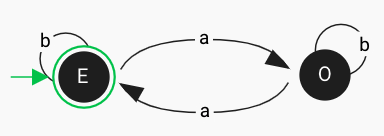
\includegraphics[width=0.7 \linewidth]{images/worksheet_8_solution_1.png}
    \end{center}

    \bigskip

    \textbf{$L_2$:}

    \bigskip

    \begin{align*}
        Q &= \{0,1,2\}\\
        \Sigma &= \{a,b\}\\
        \delta &= \begin{tabular}{|c|c|c|}
        \hline
              & a & b\\
        \hline
        $^*$0 & 1 & 1\\
        1     & 2 & 2\\
        2     & 0 & 0\\
        \hline
        \end{tabular}\\
        q_0 &= 0\\
        F &= \{0\}
    \end{align*}

    \bigskip

    Draw Diagram

    \begin{center}
    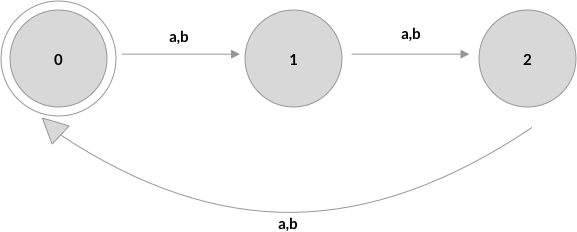
\includegraphics[width=0.7 \linewidth]{images/worksheet_8_solution_2.png}
    \end{center}

    \bigskip

    \underline{\textbf{Part 1 (Building $L_1 \cap L_2$):}}

    \bigskip

    \begin{align*}
        Q &= \{(E,0),(E,1),(E,2),(O,0),(O,1),(O,2)\}\\
        \Sigma &= \{a,b\}\\
        \delta &= \begin{tabular}{|c|c|c|}
        \hline
            & a & b\\
        \hline
        $^*$(E,0) & 1 & 1\\
        (E,1)     & 2 & 2\\
        (E,2)     & 0 & 0\\
        (O,0)     & 1 & 1\\
        (O,1)     & 2 & 2\\
        (O,2)     & 0 & 0\\
        \hline
        \end{tabular}\\
        q_0 &= (E,0)\\
        F &= \{(E,0)\}
    \end{align*}

    \bigskip

    \begin{mdframed}
    \underline{\textbf{Correct Solution:}}

    \bigskip

    \underline{\textbf{Part 1 (Building $L_1$ and $L_2$):}}

    \bigskip

    \textbf{$L_1$:}

    \bigskip

    \begin{align*}
        Q &= \{E,O\}\\
        \Sigma &= \{a,b\}\\
        \delta &= \begin{tabular}{|c|c|c|}
        \hline
          & a & b\\
        \hline
        $^*$E & O & E\\
        O & E & O\\
        \hline
        \end{tabular}\\
        q_0 &= E\\
        F &= \{E\}
    \end{align*}

    \bigskip

    Draw Diagram

    \begin{center}
    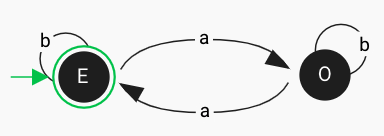
\includegraphics[width=0.7 \linewidth]{images/worksheet_8_solution_1.png}
    \end{center}

    \bigskip

    \textbf{$L_2$:}

    \bigskip

    \begin{align*}
        Q &= \{0,1,2\}\\
        \Sigma &= \{a,b\}\\
        \delta &= \begin{tabular}{|c|c|c|}
        \hline
              & a & b\\
        \hline
        $^*$0 & 1 & 1\\
        1     & 2 & 2\\
        2     & 0 & 0\\
        \hline
        \end{tabular}\\
        q_0 &= 0\\
        F &= \{0\}
    \end{align*}

    \bigskip

    Draw Diagram

    \begin{center}
    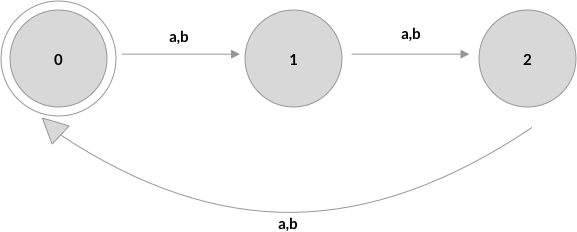
\includegraphics[width=0.7 \linewidth]{images/worksheet_8_solution_2.png}
    \end{center}

    \bigskip

    \underline{\textbf{Part 1 (Building $L_1 \cap L_2$):}}

    \bigskip

    \begin{align*}
        Q &= \{(E,0),(E,1),(E,2),(O,0),(O,1),(O,2)\}\\
        \Sigma &= \{a,b\}\\
        \delta &= \begin{tabular}{|c|c|c|}
        \hline
            & a & b\\
        \hline
        $^*$(E,0) & \color{red}(O,1)\color{black} & \color{red}(E,1)\color{black}\\
        (E,1)     & \color{red}(O,2)\color{black} & \color{red}(E,2)\color{black}\\
        (E,2)     & \color{red}(O,0)\color{black} & \color{red}(E,0)\color{black}\\
        (O,0)     & \color{red}(E,1)\color{black} & \color{red}(O,1)\color{black}\\
        (O,1)     & \color{red}(E,2)\color{black} & \color{red}(O,2)\color{black}\\
        (O,2)     & \color{red}(E,0)\color{black} & \color{red}(O,0)\color{black}\\
        \hline
        \end{tabular}\\
        q_0 &= (E,0)\\
        F &= \{(E,0)\}
    \end{align*}

    \end{mdframed}


\end{itemize}
% \bigskip

% \begin{mdframed}
% \underline{\textbf{Rough Works:}}

% \bigskip

% \begin{enumerate}[1.]
% \item Build $L_1$

% \begin{mdframed}
% \begin{align*}
%     Q &= \{E,O\}\\
%     \Sigma &= \{a,b\}\\
%     \delta &= \begin{tabular}{|c|c|c|}
%     \hline
%       & a & b\\
%     \hline
%     $^*$E & O & E\\
%     O & E & O\\
%     \hline
%     \end{tabular}\\
%     q_0 &= E\\
%     F &= \{E\}
% \end{align*}

% \bigskip

% Draw Diagram

% \begin{center}
% 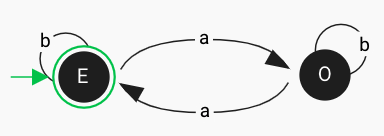
\includegraphics[width=0.7 \linewidth]{images/worksheet_8_solution_1.png}
% \end{center}

% \end{mdframed}

% \item Build $L_2$

% \begin{align*}
%     Q &= \{0,1,2\}\\
%     \Sigma &= \{a,b\}\\
%     \delta &= \begin{tabular}{|c|c|c|}
%     \hline
%           & a & b\\
%     \hline
%     $^*$0 & 1 & 1\\
%     1     & 2 & 2\\
%     2     & 0 & 0\\
%     \hline
%     \end{tabular}\\
%     q_0 &= 0\\
%     F &= \{0\}
% \end{align*}

% \bigskip

% Draw Diagram

% \begin{center}
% 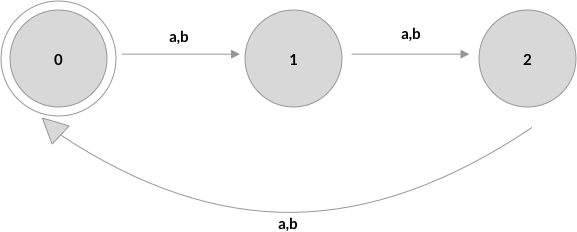
\includegraphics[width=0.7 \linewidth]{images/worksheet_8_solution_2.png}
% \end{center}

% \item Building $L_1 \cap L_2$

% \begin{align*}
%     Q &= \{0,1,2\}\\
%     \Sigma &= \{a,b\}\\
%     \delta &= \begin{tabular}{|c|c|c|}
%     \hline
%           & a & b\\
%     \hline
%     $^*$0 & 1 & 1\\
%     1     & 2 & 2\\
%     2     & 0 & 0\\
%     \hline
%     \end{tabular}\\
%     q_0 &= 0\\
%     F &= \{0\}
% \end{align*}

% \item Build $L_1 \cap L_2$

% \begin{align*}
%     Q &= \{(E,0),(E,1),(E,2),(O,0),(O,1),(O,2)\}\\
%     \Sigma &= \{a,b\}\\
%     \delta &= \begin{tabular}{|c|c|c|}
%     \hline
%           & a & b\\
%     \hline
%     $^*$(E,0) & 1 & 1\\
%     (E,1)     & 2 & 2\\
%     (E,2)     & 0 & 0\\
%     (O,0)     & 1 & 1\\
%     (O,1)     & 2 & 2\\
%     (O,2)     & 0 & 0\\
%     \hline
%     \end{tabular}\\
%     q_0 &= (E,0)\\
%     F &= \{(E,0)\}
% \end{align*}

% \end{enumerate}

% \end{mdframed}

\bigskip

\underline{\textbf{Notes:}}

\bigskip

\begin{itemize}
    \item \textbf{Deterministic Finite State Automaton (DFSA)}: is a mathematical
    method of machine which, given any input string $x$, \textbf{accepts} or
    \textbf{rejects} $x$.

    \item Applications of DFSA
    \begin{enumerate}[1.]
        \item Vending Machine
        \begin{center}
        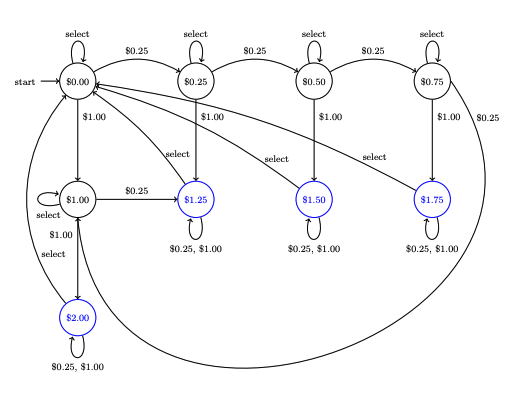
\includegraphics[width=0.8 \linewidth]{images/worksheet_8_notes_1.png}
        \end{center}

        \item Protocol analysis
        \item Text parsing
        \item Video game character behavior

        \begin{center}
        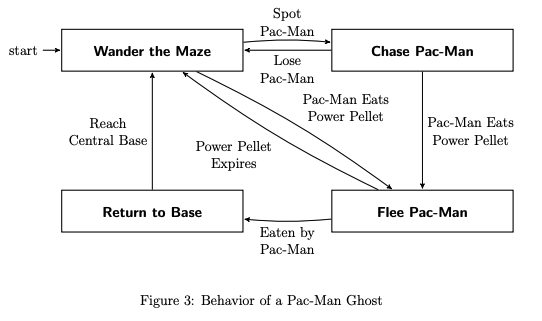
\includegraphics[width=0.8 \linewidth]{images/worksheet_8_notes_2.png}
        \end{center}

        \item Security Analysis
        \item \underline{CPU control units} (**)
        \item \underline{Natural Language Processing} (**)
        \item \underline{Speech Recognition}  (**)
    \end{enumerate}

    \item Definitions and Syntax
    \begin{center}
    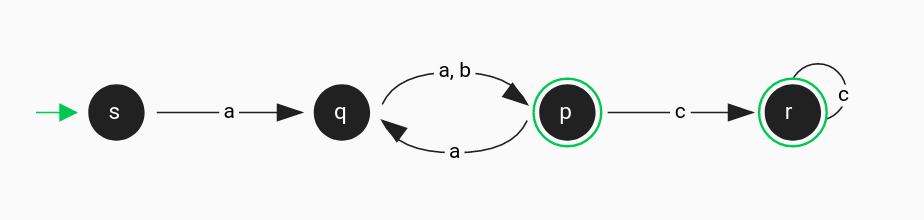
\includegraphics[width=\linewidth]{images/worksheet_8_notes_6.png}
    \end{center}
    \begin{itemize}
        \item $DFSA$ $M$ is a quintuple $M = (Q,\Sigma, q_0, F, \delta)$, where
        \begin{itemize}
            \item $Q:$ a finite set of \textbf{states}.
            \begin{itemize}
                \item Represents status of system
                \item Is represented by a black circle, i.e. s,q

                \begin{center}
                
\includegraphics[width=2cm]{images/worksheet_8_notes_8.png}
                \end{center}

                \item i.e. automatic sliding door at walmart has two states: either close or open
                \item i.e. traffic light has three states: red, yellow, green
            \end{itemize}
            \item $\Sigma:$ a finite non-empty alphabet
            \begin{itemize}
                \item is set of symbols in each transition, i.e. a, b, c

                \begin{center}
                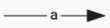
\includegraphics[width=0.3 \linewidth]{images/worksheet_8_notes_3.png}
                \end{center}
            \end{itemize}

            \item $q_0 \in Q:$ the start or initial state
            \item $\delta: Q \times \sigma \to Q:$ a transition function
            \begin{itemize}
                \item is a connection between two states.
                \item is represented by an arrow
                \begin{center}
                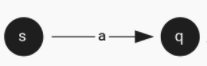
\includegraphics[width=0.4 \linewidth]{images/worksheet_8_notes_4.png}
                \end{center}
            \end{itemize}
            \item $F \subseteq Q:$ the set of accepting or final states
            \begin{itemize}
                \item Is represented by a double circle

                \begin{center}
                
\includegraphics[width=2cm]{images/worksheet_8_notes_5.png}
                \end{center}

                \item Multiple accepting states may exists
                \item Purpose: When processing ends, the output is either \textit{accept} or \textit{reject}
            \end{itemize}
        \end{itemize}
    \end{itemize}

    \item Simple Example

    \begin{itemize}
        \item Step 1

        \begin{center}
        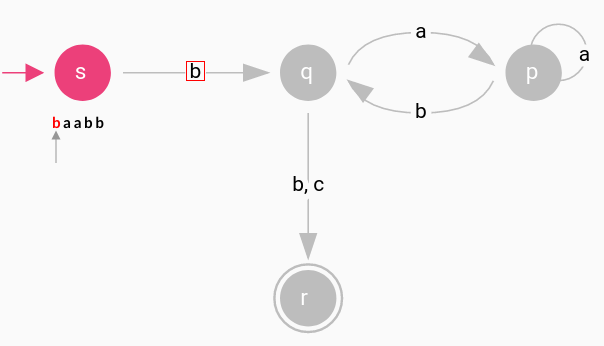
\includegraphics[width=\linewidth]{images/worksheet_8_notes_9.png}
        \end{center}

        \begin{enumerate}[1.]
            \item First symbol of the input \textbf{baabb} is \textbf{b} and the current state is \textit{s}.
            \item Ask, is there any exiting transition from \textit{s} that contains the symbol \textbf{b}?
            \item The answer is yes, so move to \textit{q}
        \end{enumerate}

        \item Step 2

        \begin{center}
        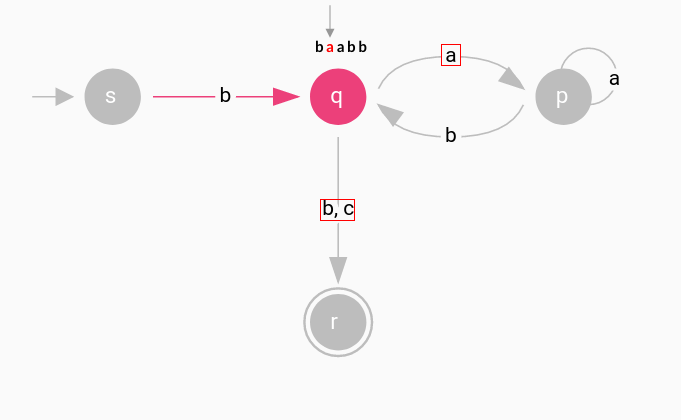
\includegraphics[width=\linewidth]{images/worksheet_8_notes_10.png}
        \end{center}

        \begin{enumerate}[1.]
            \item Next symbol of the input \textbf{baabb} is \textbf{a} and the current state is \textit{q}.
            \item Ask, is there any exiting transition from \textit{q} that contains the symbol \textbf{a} or \textbf{b,c}?
            \item The answer is yes, and it's \textbf{a}. So move to \textit{p}
        \end{enumerate}

        \item Step 3

        \begin{center}
        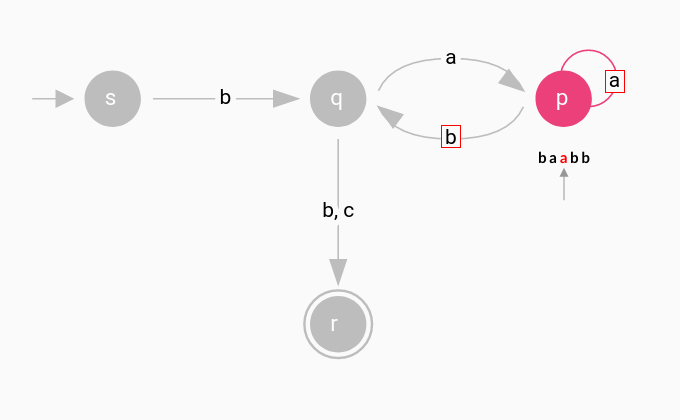
\includegraphics[width=\linewidth]{images/worksheet_8_notes_11.png}
        \end{center}

        \begin{enumerate}[1.]
            \item Next symbol of the input \textbf{baabb} is \textbf{a} and the current state is \textit{p}.
            \item Ask, is there any exiting transition from \textit{p} that contains the symbol \textbf{a} or \textbf{b}?
            \item The answer is yes, and it's \textbf{a}. So move to \textit{p}
        \end{enumerate}

        \item Step 4

        \begin{center}
        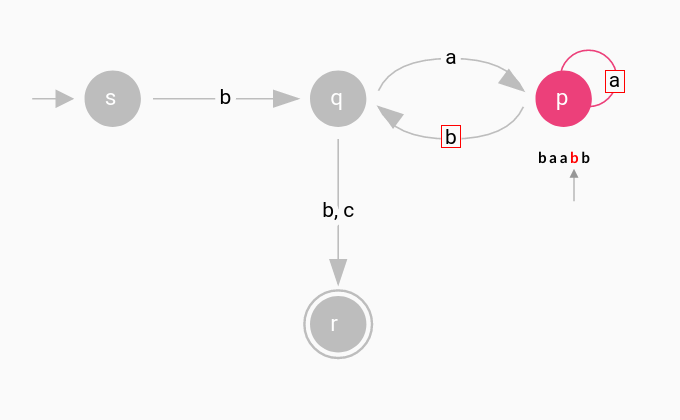
\includegraphics[width=\linewidth]{images/worksheet_8_notes_12.png}
        \end{center}

        \begin{enumerate}[1.]
            \item Next symbol of the input \textbf{baabb} is \textbf{b} and the current state is \textit{p}.
            \item Ask, is there any exiting transition from \textit{p} that contains the symbol \textbf{a} or \textbf{b}?
            \item The answer is yes, and it's \textbf{b}. So move to \textit{q}
        \end{enumerate}

        \item Step 5

        \begin{center}
        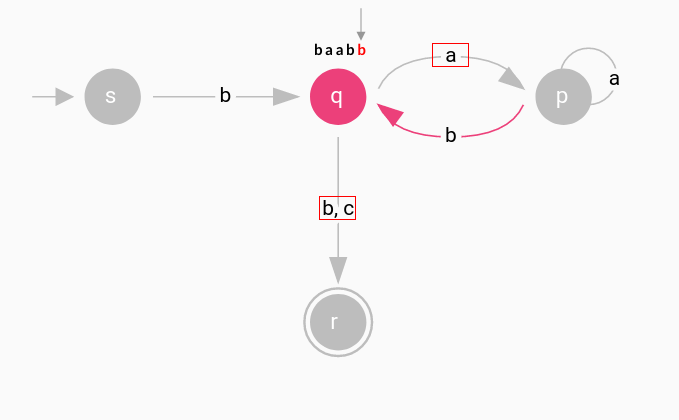
\includegraphics[width=\linewidth]{images/worksheet_8_notes_13.png}
        \end{center}

        \begin{enumerate}[1.]
            \item Next symbol of the input \textbf{baabb} is \textbf{b} and the current state is \textit{q}.
            \item Ask, is there any exiting transition from \textit{q} that contains the symbol \textbf{a} or \textbf{b,c}?
            \item The answer is yes, and it's \textbf{b}. So move to \textit{r}
        \end{enumerate}

        \item Step 6

        \begin{center}
        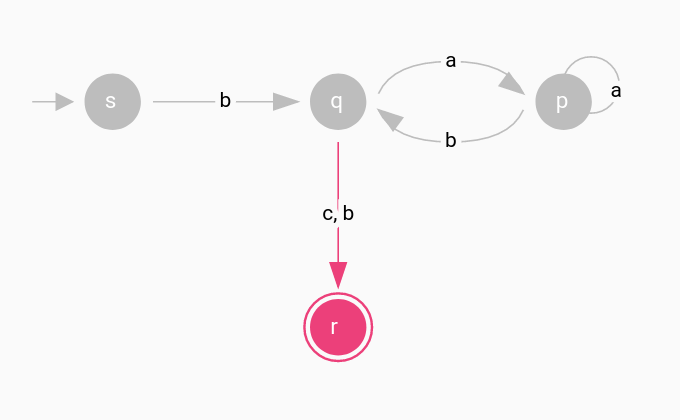
\includegraphics[width=\linewidth]{images/worksheet_8_notes_14.png}
        \end{center}

        \begin{enumerate}[1.]
            \item Next symbol of the input \textbf{baabb} is \textbf{b} and the current state is \textit{r}.
            \item Ask, if it satiesfies the accepting or final state (i.e, has the end of string been reached?). If so, the output is accept. Otherwise, it's reject.
        \end{enumerate}

    \end{itemize}

    \item Formal Languages
    \begin{itemize}
        \item is a \underline{subset} of all possible words $\Sigma *$ formed by symbols of
        alphabet $\Sigma$.

        \begin{itemize}
            \item  $\Sigma *$ is set of all possible strings over the alphabet $\Sigma$.
            \item i.e. $\Sigma = \{a,b\}$, $\Sigma* = \{a,b,aa,ab,ba,bb,aaa,aab,\cdots\}$
        \end{itemize}
        \item Example
        \begin{enumerate}[1.]
        \item $L = \{w \mid w\:\text{has at most seventeen 0's}\}$
        \item $L = \{w \mid w\:\text{has equal number of 0's and 1's}\}$
        \item $L = \{x \in \{a,b\}^* \mid \text{the number of as in $x$ is even}\}$
        \begin{itemize}
            \item * in $\{a,b\}^*$ means all possible combinations
            \item i.e. $\{a,b,aa,ab,ba,bb,aaa,baa,aba,\cdots\}$
        \end{itemize}
        \end{enumerate}
    \end{itemize}
    \item Tabular DFAs
    \begin{itemize}
        \item Example

        \begin{center}
        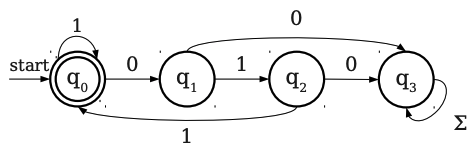
\includegraphics[width=\linewidth]{images/worksheet_8_notes_15.png}
        \end{center}

        \bigskip

        \begin{center}
        $\delta =$ \begin{tabular}{|c|c|c|}
        \hline
         & 0 & 1\\
        \hline
        $^*q_0$ & $q_1$ & $q_0$\\
        $q_1$ & $q_3$ & $q_2$\\
        $q_2$ & $q_3$ & $q_0$\\
        $q_3$ & $q_3$ & $q_3$\\
        \hline
        \end{tabular}

        \bigskip

        Note: $^*$ means it's an accepting state
        \end{center}

    \end{itemize}
\end{itemize}

\bigskip

\section*{Question 2}

\bigskip

\setcounter{equation}{0}
\underline{\textbf{Partial Solution:}}

\bigskip

\begin{enumerate}[1.]
    \item Prove that $M_1$ accepts $L_1$

    \bigskip

    First, define $\Sigma^*$ as the smallest set such that
    \begin{enumerate}
        \item $\varepsilon \in \Sigma^*$
        \item $s \in \Sigma^* \Rightarrow sa \in \Sigma^* \land sb \in \Sigma^*$
    \end{enumerate}

    \bigskip

    I will prove that $M_1$ accepts $L_1$.

    \bigskip

    Define $P(s)$ as:

    \begin{align}
        P(s):\delta^*(E,s) &= \begin{cases}
            E & \text{if $s$ has an even number of $as$}\\
            O & \text{if $s$ has an even number of $as$}
        \end{cases}
    \end{align}

    I will prove $\forall s \in \Sigma^*$, $P(s)$ by structural induction.

    \begin{enumerate}[1.]
        \item Basis Case

        \bigskip

        $\vert \varepsilon \vert = 0$, an even number, and $\delta^*(E,\varepsilon) = E$
        so the implication in the first line of the invariant is true in this case.
        Also since $\vert \varepsilon \vert$ is not odd, the implication in the second
        line of the invariant is vacuously true. So $P(\varepsilon)$ holds.

        \item Inductive Step

        \bigskip

        Let $s \in \Sigma^*$ and assume $P(s)$. I will show that $P(sa)$ and $P(sb)$
        follow. There are two cases to consider:

        \begin{enumerate}[1.]
            \item Case $sa$

            \bigskip

            Then,

            \begin{align}
            \delta^*(E,sa) = \delta(\delta^*(E,s),a) &= \begin{cases}
                \delta(E,a) & \text{if $s$ has even number of $as$}\\
                \delta(O,a) & \text{if $s$ has odd number of $as$}\\
            \end{cases} & [\text{By $P(s)$}]\\
            &= \begin{cases}
                O & \text{if $sa$ has odd number of $as$}\\
                E & \text{if $sa$ has even number of $as$}\\
            \end{cases} & [\text{One more $a$}]
            \end{align}

            \item Case $sb$ (Let's first start with this)

            \begin{mdframed}
            Then,

            \bigskip

            \begin{align}
            \delta^*(E,sb) = \delta(\delta^*(E,s),b) &= \begin{cases}
                \delta(E,b) & \text{if $s$ has even number of $as$}\\
                \delta(O,b) & \text{if $s$ has odd number of $as$}\\
            \end{cases} & [\text{By $P(s)$}]\\
            &= \begin{cases}
                E & \text{if $sb$ has odd number of $as$}\\
                O & \text{if $sb$ has even number of $as$}\\
            \end{cases} & [\text{One more $b$}]
            \end{align}

            \end{mdframed}

            \bigskip

            So $P(sa)$ and $P(sb)$ follow.

            \bigskip

            The first line of the invariant ensures that all strings with an even number
            $as$ are accepted. The contrapositive of the second line of the invariant
            ensures that any string that does not drive the machine to state $O$ does
            not have an odd number of $as$, in other words all strings that drive
            the machine to state $E$ have an even number of $as$. So $M_1$ accepts $L_1$.

        \end{enumerate}
    \end{enumerate}

    \item Prove that $M_2$ accepts $L_2$

    \bigskip

    Define $P(s)$ as:

    \begin{align}
        P(s): \delta^*(0,s) = \begin{cases}
            0 & \text{if $\vert s \vert \equiv 0 \mod (3)$}\\
            1 & \text{if $\vert s \vert \equiv 1 \mod (3)$}\\
            2 & \text{if $\vert s \vert \equiv 2 \mod (3)$}\\
        \end{cases}
    \end{align}

    I prove $\forall s \in \Sigma^*$, $P(s)$ by structural induction.

    \bigskip

    \begin{enumerate}[1.]
        \item Basis Case (Let's give this a shot)

        \begin{mdframed}
        I need to prove $P(\varepsilon)$ holds.

        \bigskip

        Let $\varepsilon \in \Sigma^*$.

        \bigskip

        Then, since $\vert \varepsilon \vert = 0$, $\delta^*(0,\varepsilon) = 0$.

        \bigskip

        So, the implication of the first line is true in this case.

        \bigskip

        Also, since $\vert \varepsilon \vert \not\equiv 1 \mod 3$, the implication
        of second line is vacuously true in this case.

        \bigskip

        Also, since $\vert \varepsilon \vert \not\equiv 2 \mod 3$, the implication
        of third line is vacuously true in this case.

        \bigskip

        Thus, $P(\varepsilon)$ holds.

        \end{mdframed}

        \item Inductive Step (Let's also try this)

        \begin{mdframed}

            Let $s \in \Sigma^*$ and assume $P(s)$. Let $@ \in \{a,b\}$. I will
            show $P(s@)$ follows.

            \bigskip

            Starting from $\delta^*(0,s@)$, we have

            \begin{align}
            \delta^*(0,s@) &= \begin{cases}
                \delta(0,@) & \text{if $\vert s \vert \equiv 0 \mod 3$}\\
                \delta(1,@) & \text{if $\vert s \vert \equiv 1 \mod 3$}\\
                \delta(2,@) & \text{if $\vert s \vert \equiv 2 \mod 3$}
            \end{cases} & [\text{By $P(s)$}]\\
            &= \begin{cases}
                0 & \text{if $\vert s \vert \equiv 0 \mod 3$}\\
                1 & \text{if $\vert s \vert \equiv 1 \mod 3$}\\
                2 & \text{if $\vert s \vert \equiv 2 \mod 3$}
            \end{cases} & [\text{Since adding a char doesn't change inv. cond.}]\\
            \end{align}

            \bigskip

            Thus, $P(s@)$ follows.

            \bigskip

            The first line of the invariant ensures that all strings with length
            equivalent to $0 \mod 3$ or multiples of 3 are accepted. The contrapositive
            of the second line of the invariant ensures that any string that does
            not drive the machine to state 1 does not have length equivalent to
            $1 \mod 3$. The contrapositive of the third line of the invariant
            ensures that any string that does not drive the machine to state 2 does
            not have length equivalent to $2 \mod 3$.

            \bigskip

            So, $M_2$ accepts $L_2$.
        \end{mdframed}

    \end{enumerate}

    \item Prove that $M_{1\land2}$ accepts $L_1 \cap L_2$

    \bigskip

    Denote the states for $M_1$ as $Q_1$, the states for $M_2$ as $Q_2$, their
    respective transition functions as $\delta_1$ and $\delta_2$, and the transition
    function for $M_{1\land 2}$ and the transition function for $M_{1\land 2}$ as $\delta_{1 \land 2}$.
    Inspection of $\delta_{1 \land 2}$ shows that if $(q_1,q_2,c) \in Q_1 \times Q_2 \times \Sigma$,
    then $\delta_{1\land 2}((q_1,q_2),c) = (\delta_1(q_1,c),\delta_2(q_2,c))$. Thus,
    the following invariant follows by simplying taking conjunctions of the invariants
    of the component machines, for any $s \in \Sigma^*$.

    \begin{align}
        P(s):\delta^*((E,0),s) &= \begin{cases}
            (E,0) & \text{if $s$ has an even number of $as \land \vert s \vert \equiv 0 \mod 3$}\\
            (E,1) & \text{if $s$ has an even number of $as \land \vert s \vert \equiv 1 \mod 3$}\\
            (E,2) & \text{if $s$ has an even number of $as \land \vert s \vert \equiv 2 \mod 3$}\\
            (O,0) & \text{if $s$ has an even number of $as \land \vert s \vert \equiv 0 \mod 3$}\\
            (O,1) & \text{if $s$ has an even number of $as \land \vert s \vert \equiv 1 \mod 3$}\\
            (O,2) & \text{if $s$ has an even number of $as \land \vert s \vert \equiv 2 \mod 3$}\\
        \end{cases}
    \end{align}

    \bigskip

    The implication on the first line ensures that all strings with an even number
    of $as$ and a length that is a multiple of 3 end up in state $(e,0)$. The
    contrapositive of the implications on the other lines ensure that nay string that does
    not derive the machine to one of those 5 states must have an even number of $as$
    and a length that is a multiple of 3. Hence $M_{1 \land 2}$ accepts
    $L_1 \cap L_2$.
    \end{enumerate}


\end{document}